\documentclass[11pt]{beamer}
\usetheme{metropolis}  
\usecolortheme{beaver}
\usepackage{hyperref}
\usepackage{bigints}
\usepackage{amsmath}
\usepackage{framed}
\usepackage{multicol}
\title{T\'opicos de investigaci\'on  CM072}
 \usepackage[spanish]{babel}
 \decimalpoint
\date{\today}
\author{C\'esar Lara Avila}
\institute{\url{https://github.com/C-Lara}}
\begin{document}
  \maketitle
  \section{2. Teoria del aprendizaje }
  
\begin{frame}{Ejemplo de regresi\'on :}
\begin{columns}
\begin{column}{0.5\textwidth}
\textbf{Conjunto de datos:}  $10$ puntos $(X,Y)$ generados de una funci\'on \text{seno} con ruido.

\vspace{0.2cm}
		
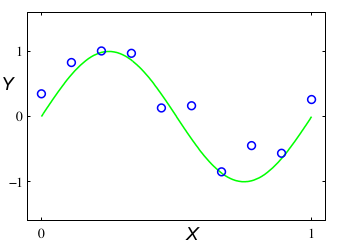
\includegraphics[scale= 0.45]{TA1.png}
	\end{column}
	\begin{column}{0.5\textwidth}  
		\begin{itemize}
			\item \textbf{Regresi\'on}
			\begin{itemize}
				\item $f: X \rightarrow Y$
				\item $X = \mathbb{R}$
				\item $Y = \mathbb{R}$
			\end{itemize}
			\vspace{3.6cm}
			
		\end{itemize}
	\end{column}
\end{columns}
	
\end{frame}

\begin{frame}{Polinomios de  grado M}
		
\textbf{?`Que tal si dejamos que $f$ sea un polinomio de grado $M$?}

\vspace{0.3cm}

\begin{columns}
\begin{column}{0.3\textwidth}
			
\begin{itemize}
	\item ?` Cu\'al es el \textbf{mejor}?
\end{itemize}
	\end{column}
	\begin{column}{0.7\textwidth}  
		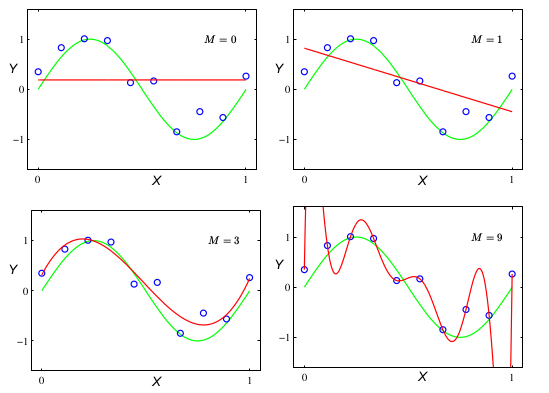
\includegraphics[scale= 0.35]{TA2.png}
	\end{column}
\end{columns}

\end{frame}

\begin{frame}{Espacio de hip\'otesis: Polinomios de grado N}

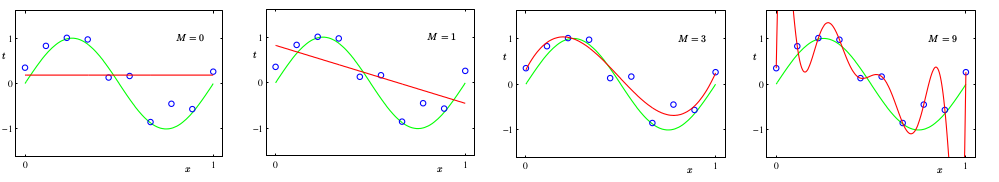
\includegraphics[scale= 0.33]{TA3.png}

\vspace{0.2cm}

\begin{columns}
\begin{column}{0.55\textwidth}
	
\vspace{0.3cm}


\scriptsize{Medimos el error usando una funci\'on de p\'erdida $L(y, \hat{y})$. 
	
\vspace{0.2cm}

Para la regresi\'on, una opci\'on com\'un es la p\'erdida al cuadrado:
	
\vspace{0.2cm}


$L(y_i, f(x_i)) = (y_i -f(x_i))^2$

\vspace{0.2cm}

La p\'erdida emp\'irica de la funci\'on $f$ aplicada a los datos de entrenamiento es entonces:

\vspace{0.2cm}


$\displaystyle \frac{1}{N}\sum_{i =1}^{N}L(x_i, f(x_i)) = \frac{1}{N}\sum_{i =1}^{N}(y_i -f(x_i))^2$
}
\end{column}
\begin{column}{0.45\textwidth} 
	
\quad \scriptsize\textbf{Curva de aprendizaje}
\vspace{0.2cm}
 
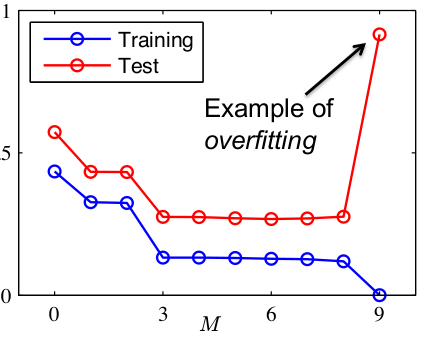
\includegraphics[scale= 0.3]{TA4.png}
\quad \scriptsize\textbf{Medida de la complejidad del modelo}

\end{column}
\end{columns}
\end{frame}

\begin{frame}{Clasificaci\'on binaria}
\begin{columns}
\begin{column}{0.61\textwidth}
		
\begin{itemize}
\item \textcolor{blue}{\textbf{Entradas:}} Email, 
\item \textcolor{blue}{\textbf{Salida:}} Spam/Ham
\item \textcolor{blue}{\textbf{Preparaci\'on:}}

\begin{itemize}
\item  \scriptsize{Obtenemos una gran colecci\'on de correos electr\'onicos de ejemplo, cada uno etiquetado como \texttt{spam} o \text{ham}.}
\item \scriptsize{Nota: alguien tiene que manejar las etiquetas de todos estos datos!.}
\item \scriptsize{Quieres aprender a predecir etiquetas de nuevos, futuros correos electr\'onicos.}
\end{itemize}
\item \textcolor{blue}{\textbf{Caracter\'isticas:}} \scriptsize{Los atributos utilizados para tomar la decisi\'on de \texttt{ham/spam}}.
\begin{itemize}
\item \scriptsize{Palabras: GRATIS!}
\item  \scriptsize{Patrones de texto: $\$dd$ , CAPS}
\item  \scriptsize{Sin texto: SenderInContacts}
\end{itemize}
\end{itemize}
\end{column}
\begin{column}{0.49\textwidth}  
\begin{framed}
\scriptsize{Estimado Estudiante.}

\vspace{0.2cm}

\tiny {Debo solicitar su confianza en esta transacci\'on, esto es en virtud de su naturaleza como totalmente confidencial y secreto. ...\huge$\times$
}
\end{framed}
\begin{framed}
\tiny{PARA SER REMOVIDO DE CORREOS FUTUROS,  PONER \textbf{REMOVER} EN EL ASUNTO MENSAJE.

$99$ MILLONES DE DIRECCIONES DE CORREO ELECTRONICO POR SOLO $ 59$ SOLES. \huge$\times$}
\end{framed}
\begin{framed}
\tiny{ Elimin\'e mi archivo configuraci\'on  \texttt{.gitconfig} Linux. Tuve que utilizar \texttt{git reset}, con un poco de suerte completar\'e las tareas y asignaciones bajo cambio de fechas. \huge \checkmark}
\end{framed}
\end{column}
\end{columns}
\end{frame}

\begin{frame}{El algoritmo del perceptron}
\begin{itemize}
	\item $1957$: El algoritmo perceptron fue inventado por Frank Rosenblatt.
	\item Construido sobre el trabajo de Hebbs ($1949$); tambi\'en desarrollado por Widrow-Hoff ($1960$).
	\item El algoritmo perceptr\'on es un \textcolor{orange}{algoritmo de descenso por gradiente} y puede necesitar que se le presente m\'as de una vez un determinado patr\'on del conjunto de  entrenamiento. 
	
	\item El \textcolor{blue}{\textbf{teorema de convergencia del perceptr\'on}} demuestra que si las muestras son linealmente separables, el algoritmo converge a una soluci\'on adecuada.
\end{itemize}
\end{frame}

\begin{frame}{Clasificadores lineales}
\begin{itemize}
\small{
\item Las entradas son \textcolor{orange}{\textbf{valores de caracter\'isticas}}.

\item Cada caracter\'istica tiene un \textcolor{orange}{\textbf{peso}}.

\item  La suma es la \textcolor{orange}{\textbf{activaci\'on}}.

\[
\text{activacion}_w(x) = \sum_iw_i\cdot f_i(x) = w\cdot f(x)
\]

\item \textcolor{blue}{Si la activaci\'on es:}
\begin{columns}
\begin{column}{0.55\textwidth}
	
\qquad - \small {Positiva, salida de la clase 1}
			
\qquad - \small {Negativa, salida de la clase 2 }
\end{column}
	\begin{column}{0.45\textwidth}  
		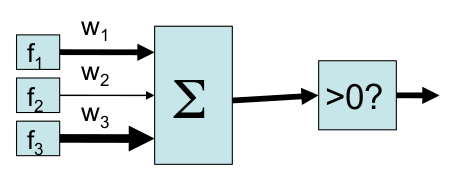
\includegraphics[scale= 0.32]{TA10.png}
		
	\end{column}
\end{columns}

}
\end{itemize}
\end{frame}

\begin{frame}{Ejemplo: Spam}
\small{Imagina 3 caracter\'isticas (el spam es una clase positiva):
\begin{enumerate}
	\item \texttt{free} (n\'umero de ocurrencias de \texttt{free}).
	\item \texttt{money} (ocurrencias de \texttt{money})
	\item BIAS (interceptar, siempre tiene el valor 1)
\end{enumerate}

	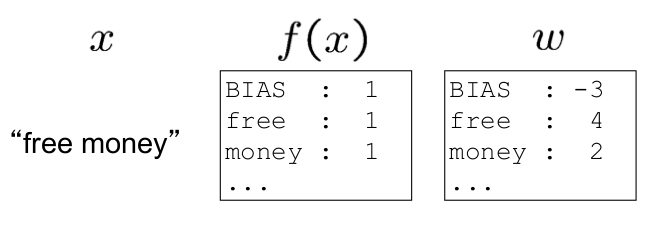
\includegraphics[scale= 0.28]{TA11.png}
	
\[
\sum_{i}w_i\cdot f_i(x) = (1)(-3) + (1)(4) + (1)(2) + \cdots = 3
\]
}


\qquad \Large{\textcolor{blue}{$\mathbf{w. f(x) > 0} \rightarrow  \textbf{ SPAM}$ }}.

\end{frame}

\begin{frame}{Regla de decisi\'on binaria}
\small{
\begin{itemize}
	\item En el espacio de los vectores de caracter\'isticas
	\begin{itemize}
		\item Ejemplos son los puntos
		\item  Cualquier vector de peso es un hiperplano
		\item  Un lado corresponde a $Y = +1$
		\item  Otro corresponde a $Y = -1$
	\end{itemize}
	
\end{itemize}
\begin{columns}
	\begin{column}{0.35\textwidth}
		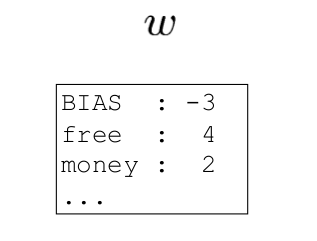
\includegraphics[scale= 0.32]{TA12.png}
	\end{column}
	\begin{column}{0.65\textwidth}  
		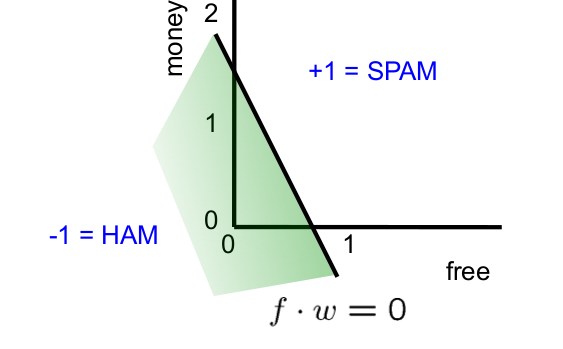
\includegraphics[scale= 0.32]{TA13.png}
		
	\end{column}
\end{columns}

	
	
	}
\end{frame}
\begin{frame}{El algoritmo del perceptron}
\begin{columns}
	\begin{column}{0.7\textwidth}
\begin{itemize}
\item Empezamos con un vector peso $\mathbf{0}$.
\item Para cada instancia de entrenamiento $(x_i, y_i)$:
\begin{itemize}
	\item Clasificamos con los pesos actuales
	
		\[
		y = \begin{cases}
		+1 \ \text{si}\ w\cdot f(x_i) \geq 0 \\
		-1 \ \text{si}\ w\cdot f(x_i) < 0 
		\end{cases}
		\]
	\item Si es correcto (es decir, $y = y_i$), no hay cambio!.
\item Si es incorrecto: actualizamos
\[
w = w + y_if(x_i)
\]
\end{itemize}
\end{itemize}	
	\end{column}
	\begin{column}{0.3\textwidth}  
		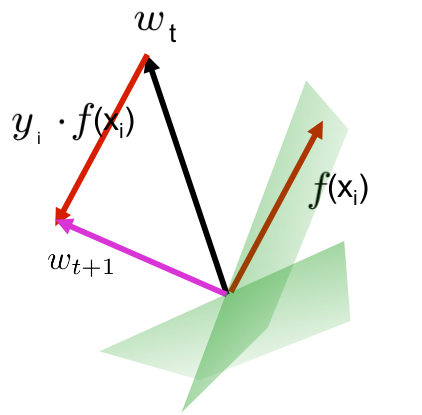
\includegraphics[scale= 0.25]{TA9.png}
	\end{column}
\end{columns}
\end{frame}
\begin{frame}{Preguntas acerca de un algoritmo de aprendizaje}
\begin{itemize}
	\item ?`Cu\'al es el tiempo de ejecuci\'on del algoritmo perceptron?.
	
	\item Si existe un vector de peso con peque\~no error de entrenamiento, puede el perceptr\'on encontrar el error?.
	
	\item  ?`Qu\'e tan bien el clasificador resultante generaliza los datos no vistos?.
\end{itemize}

\vspace{2.0cm}

\end{frame}
\begin{frame}{Separabilidad lineal}
\small{ 
$\exists \mathbf{w}$ tal que $\forall t$\qquad $y_t(\mathbf{w}\cdot \mathbf{x}_t) \geq \gamma >  0$

donde $\gamma$ es llamado el \textcolor{orange}{margen funcional} con respecto al conjunto de entrenamiento.
	
}

\vspace{0.5cm}

\begin{columns}
	\begin{column}{0.6\textwidth}
		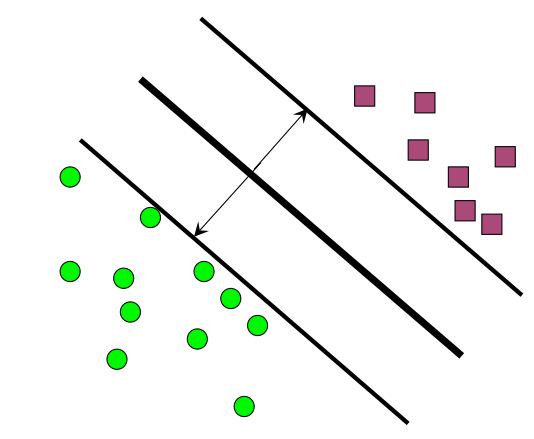
\includegraphics[scale= 0.28]{TA8.png}	
	\end{column}
	\begin{column}{0.4\textwidth}  
\small{
	Equivalentemente, para $y_t = +1$,
	
	\[
	w\cdot x_t \geq \gamma
	\]
	
	y para $y_t = -1$,
	
		\[
		w\cdot x_t \leq \gamma
		\]
	
	
}
	\end{column}
\end{columns}
\end{frame}


\begin{frame}{Error para el perceptr\'on}
\small{
\begin{itemize}
	\item Supongamos que el conjunto de datos $D$ es linealmente separable con un margen geom\'etrico $\gamma$,
	
	\[
	\exists w^{*}  \text{tal que} \quad \Vert w^{*} \Vert = 1 \quad \text{y}\quad  \forall t \ y_t(w^{*}\cdot x_t) \geq \gamma
	\]
	
	\item Asumimos que $\Vert x_t \Vert \leq R,\ \forall t$
\end{itemize}

\vspace{0.3cm}

\textcolor{violet}{\textbf{Teorema}}


El n\'umero m\'aximo de errores cometidos por el algoritmo perceptr\'on est\'a limitado por $R^2/\gamma^2$.
	
	
}
\end{frame}
\begin{frame}{Problemas con el algoritmo  perceptron}
\begin{columns}
	\begin{column}{0.55\textwidth}
\begin{itemize}
\item \small {Si los datos no son linealmente separables, no hay garant\'ias de convergencia o precisi\'on de entrenamiento.}

\item \small {Incluso si los datos de entrenamiento son linealmente separables, perceptr\'on puede ser sobrecargado}

\item \small {El perceptr\'on promedio es una modificaci\'on algor\'itmica que ayuda con ambos problemas}
\begin{itemize}
	\item \scriptsize{Promedio de los vectores de peso a trav\'es de todas las iteraciones.}
\end{itemize}
\end{itemize}
	
	\end{column}
	\begin{column}{0.45\textwidth}  
		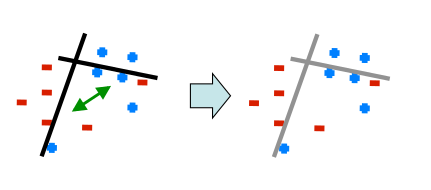
\includegraphics[scale= 0.32]{TA6.png}
		
	\vspace{0.8cm}
	
		
	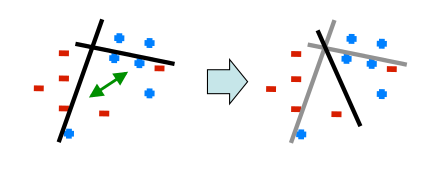
\includegraphics[scale= 0.32]{TA7.png}
	\end{column}
\end{columns}
\end{frame}
\end{document}